\section{Auswertung}
\label{sec:Auswertung}

Im Folgendem wird anhand eines Strömungsrohres die Fließgeschwindigkeit und
das Strömungsprofil als Funktion des Dopplerwinkels untersucht.


\subsection{Vorbereitungsaufgabe}

Die Dopplerwinkel berechnen sich nach der Formel
\begin{equation}
    \alpha = 90° - \text{arcsin}\left(\text{sin} \theta \frac{c_L}{c_P}\right).
\end{equation}
Daraus folgt für die drei Prismenwinkel die Dopplerwinkel in \autoref{tab:vorbereitung}.
\begin{table}
  \centering
  \caption{Der Dopplerwinkel zu dem jeweiligen Prismenwinkel.}
  \label{tab:vorbereitung}
  \begin{tabular}{c c}
    \toprule
    $\theta$ &  $\alpha$ \\ 
    \midrule
      $\qty{15}{°}$ & $\qty{80.06}{°}$ \\
      $\qty{30}{°}$ & $\qty{70.53}{°}$ \\
      $\qty{45}{°}$ & $\qty{54.74}{°}$ \\
    \bottomrule
  \end{tabular}
\end{table}


\subsection{Bestimmung der Strömungsgeschwindigkeit}

Wie in \autoref{tab:winkel} dargestellt, werden aus den Messdaten die Frequenzverschiebung 
$\increment \nu = \nu_\text{Mittel} - \nu_\text{max}$ berechnet und gegen die Strömungsgeschwindigkeit aufgetragen.
Dabei wird von einer Maximalleistung von $\text{P}_\text{max} = \qty{9000}{W} = \qty{10}{\liter\per\minute}$ ausgegangen, 
nach der die Leistung der Zentrifugalpumpe prozentual variiert wird.
\begin{table}
  \centering
  \caption{Die aus den Messdaten errechneten Frequenzverschiebungen für drei Prismenwinkel.}
  \label{tab:winkel}
  \begin{tabular}{c c c c}
    \toprule
    \multicolumn{4}{c}{$\increment \nu \mathbin{/} \mathrm{Hz}$} \\
    \cmidrule(lr){1-4}
    
    \multicolumn{1}{c}{$P \mathbin{/} \% $} &
    \multicolumn{3}{c}{$\qty{15}{°} \quad \qty{30}{°} \quad \qty{60}{°}$} \\
    \cmidrule(lr){1-1}\cmidrule(lr){2-4}

       33 &  34 &  -45 &  45 \\
       50 &  60 & -124 &  74 \\
       66 & 140 & -186 & 192 \\
       83 & 202 & -377 & 321 \\
      100 & 221 & -552 & 803 \\
    \bottomrule
  \end{tabular}
\end{table}

Hierbei ist anzumerken, dass der Prismenwinkel bei $\theta  = \qty{30}{°}$ aufgrund der Durchschallungsrichtung negative Frequenzverschiebungen hervorbringt,
weswegen im Folgenden nur der Betrag $| \increment \nu |$ betrachtet wird.
Die Strömungsgeschwindigkeit ergibt sich mithilfe von \autoref{eq:freqvers} zu
\begin{equation}
  v = \frac{| \increment \nu | \cdot c}{2 \nu_0 \cdot \cos (\alpha)}
\end{equation}
mit der verwendeten Ultraschallsonde $\nu_0 = \qty{2}{MHz}$.
Die daraus resultierenden Strömungsgeschwindigkeiten sind in \autoref{tab:strömung} dargestellt.
\begin{table}
  \centering
  \caption{Die aus den Messdaten errechneten Frequenzverschiebungen für drei Prismenwinkel.}
  \label{tab:strömung}
  \begin{tabular}{c c c c}
    \toprule
    \multicolumn{4}{c}{$v \mathbin{/} \mathrm{ms^{-1}}$} \\
    \cmidrule(lr){1-4}
    
    \multicolumn{1}{c}{$P \mathbin{/} \% $} &
    \multicolumn{3}{c}{$\qty{15}{°} \qquad \qty{30}{°} \qquad \qty{60}{°}$} \\
    \cmidrule(lr){1-1}\cmidrule(lr){2-4}

       33 & 0,148 &   0,101 &    0,096 \\
       50 & 0,261 &   0,279 &    0,249 \\
       66 & 0,608 &   0,418 &    0,417 \\
       83 & 0,877 &   0,848 &    0,731 \\
      100 & 0,960 &   1,241 &    1,043 \\
    \bottomrule
  \end{tabular}
\end{table}

Nun wird das Verhältnis von $\frac{\increment \nu}{\cos (\alpha)}$ in Abhängigkeit der Strömungsgeschwindigkeit
$\nu$ in den folgenden Tabellen aufgetragen.
\begin{figure}
  \centering
  
  \begin{subfigure}{0.65\columnwidth}
    \centering
    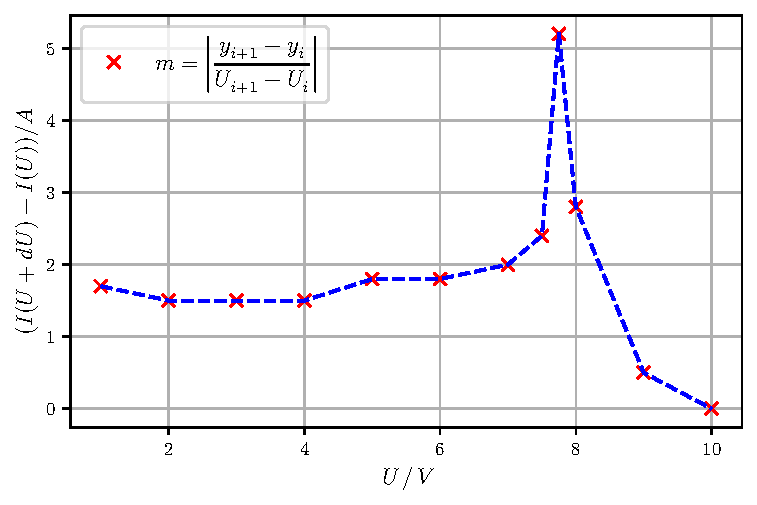
\includegraphics[width=\textwidth]{plot1.pdf}
    \caption{Frequenzverschiebung in Abhängigkeit der Strömungsgeschwindigkeit für $\theta = \qty{15}{°}$.}
    \label{fig:w15}
  \end{subfigure}
  
  \medskip
  
  \begin{subfigure}{0.65\columnwidth}
    \centering
    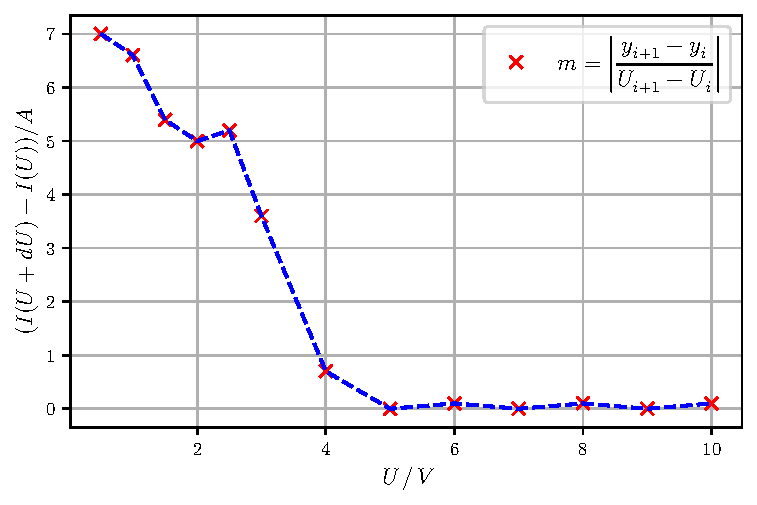
\includegraphics[width=\textwidth]{plot2.pdf}
    \caption{Frequenzverschiebung in Abhängigkeit der Strömungsgeschwindigkeit für $\theta = \qty{30}{°}$.}
    \label{fig:w30}
  \end{subfigure}
  
  \medskip
  
  \begin{subfigure}{0.65\columnwidth}
    \centering
    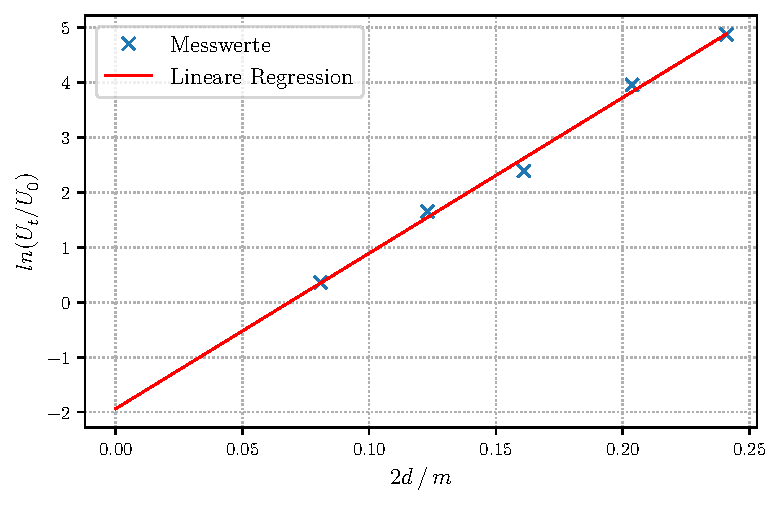
\includegraphics[width=\textwidth]{plot3.pdf}
    \caption{Frequenzverschiebung in Abhängigkeit der Strömungsgeschwindigkeit für $\theta = \qty{60}{°}$.}
    \label{fig:w60}
  \end{subfigure}

  \caption{Die Ausgleichsgeraden der Abhängigkeiten für drei Winkel von $\theta$}
  \label{fig:winkel}
\end{figure}


\subsection{Bestimmung des Strömungsprofils}

Zur Untersuchung des Strömungsprofils wird bei einem Prismenwinkel von $\theta = \qty{15}{°}$
für zwei Leistungen der Zentrifugalpumpe die Strömungsgeschwindigkeit und Streuintensität gemessen.
Dabei entspricht eine Messtiefe von $\qty{4}{\micro\second}$ in der Dopplerflüssigkeit $\qty{10}{\milli\meter}$, 
wodurch $x_\text{sec}$ in $x_\text{mm}$ für das Innenrohr mit dem Innendurchmesser von $\qty{10}{\milli\meter}$ umgerechnet werden kann. 
Die Messdaten beider Leistungen sind in \autoref{tab:profil} dargestellt.

\begin{table}[H]
  \centering
  \caption{Die Messdaten der Frequenzverschiebungen und Streuintensitäten für je 75$\%$ und 45$\%$ Leistung.}
  \label{tab:profil}

  \begin{tabular}{c c}   % top level tables, with 2 columns
      \begin{tabular}{c c c} 
          \hline
          \toprule
           & $P = \qty{75}{\percent}$ & \\
          \midrule
          $x_\text{mm} \mathbin{/} \unit{\milli\meter}$ &
          $v \mathbin{/} \mathrm{cm s^{-1}}$ &
          $I_\text{S} \mathbin{/} \mathrm{1000 \, V^2 s^{-1}}$ \\
          \midrule
          0,00 &  0,0 &  20,0 \\
          0,75 & 45,1 &  40,0 \\
          1,50 & 53,1 &  59,0 \\
          2,25 & 58,4 &  65,0 \\
          3,00 & 66,3 &  74,0 \\
          3,75 & 66,3 &  82,0 \\
          4,50 & 63,7 &  99,0 \\
          5,25 & 53,1 & 117,0 \\
          6,00 & 53,1 & 140,0 \\
          6,75 & 42,4 & 130,0 \\
          7,50 & 37,1 &  88,0 \\
          8,25 & 31,8 &  52,0 \\
          9,00 &  0,0 &  27,0 \\
          9,75 &  0,0 &  19,0 \\
         10,50 &  0,0 &  17,0 \\
 
          \bottomrule
          \hline
      \end{tabular} &  % starting rightmost sub table

      % table 2
      \begin{tabular}{c c c} 
          \hline
          \toprule
          & $P = \qty{45}{\percent}$ & \\
          \midrule
          $x_\text{mm} \mathbin{/} \unit{\milli\meter}$ &
          $v \mathbin{/} \mathrm{cm s^{-1}}$ &
          $I_\text{S} \mathbin{/} \mathrm{1000 \, V^2 s^{-1}}$ \\
          \midrule
          0,00 &  0,0 &   5,0 \\
          0,75 &  0,0 &  18,0 \\
          1,50 &  0,0 &  24,0 \\
          2,25 & 26,5 &  51,0 \\
          3,00 & 26,5 &  60,0 \\
          3,75 & 26,5 &  73,0 \\
          4,50 & 26,5 &  81,0 \\
          5,25 & 23,9 & 102,0 \\
          6,00 & 21,2 &  71,0 \\
          6,75 & 18,6 &  69,0 \\
          7,50 & 15,9 &  39,0 \\
          8,25 &  0,0 &  14,0 \\
          9,00 &  0,0 &   9,0 \\
          9,75 &  0,0 &   8,0 \\
         10,50 &  0,0 &   7,0 \\
          \bottomrule
          \hline
      \end{tabular} \\
  \end{tabular}

\end{table}

Mithilfe dieser Daten wird für beide Geschwindigkeiten jeweils die Momentangeschwindigkeit und Streuintensität
in Abhängigkeit der Messtiefe $x$ in \autoref{fig:profile} aufgetragen.
\begin{figure}[H]
  \centering
  
  \begin{subfigure}{0.49\columnwidth}
  \centering
  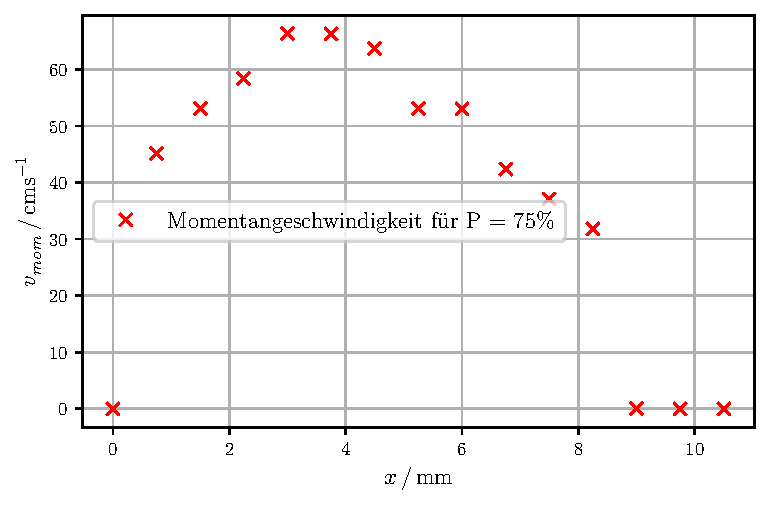
\includegraphics[width=\textwidth]{plot4.pdf}
  \caption{Die Momentangeschwindigkeit für 75$\%$.}
  \label{fig:p4}
  \end{subfigure}\hfill
  \begin{subfigure}{0.49\columnwidth}
  \centering
  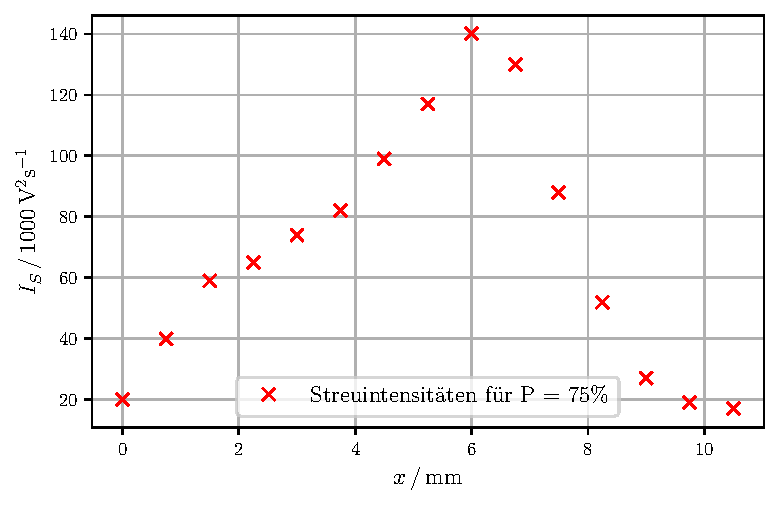
\includegraphics[width=\textwidth]{plot5.pdf}
  \caption{Die Streuintensität für 75$\%$.}
  \label{fig:p5}
  \end{subfigure}
  
  \medskip
  
  \begin{subfigure}{0.49\columnwidth}
  \centering
  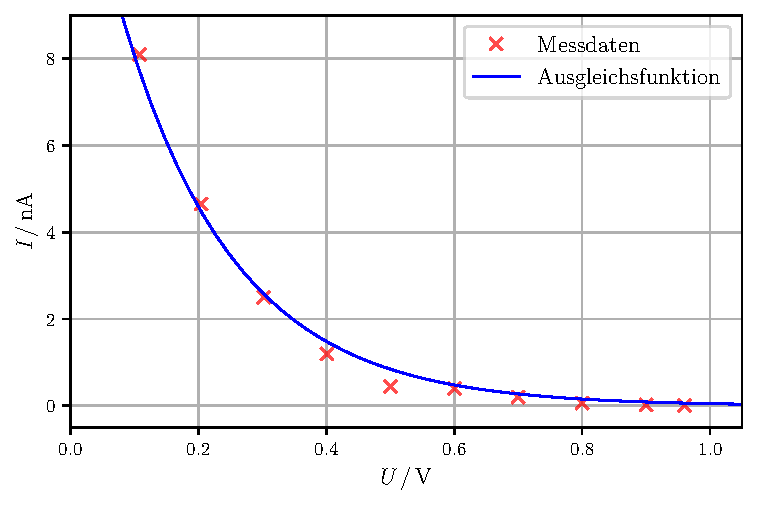
\includegraphics[width=\textwidth]{plot6.pdf}
  \caption{Die Momentangeschwindigkeit für 45$\%$.}
  \label{fig:p6}
  \end{subfigure}\hfill
  \begin{subfigure}{0.49\columnwidth}
  \centering
  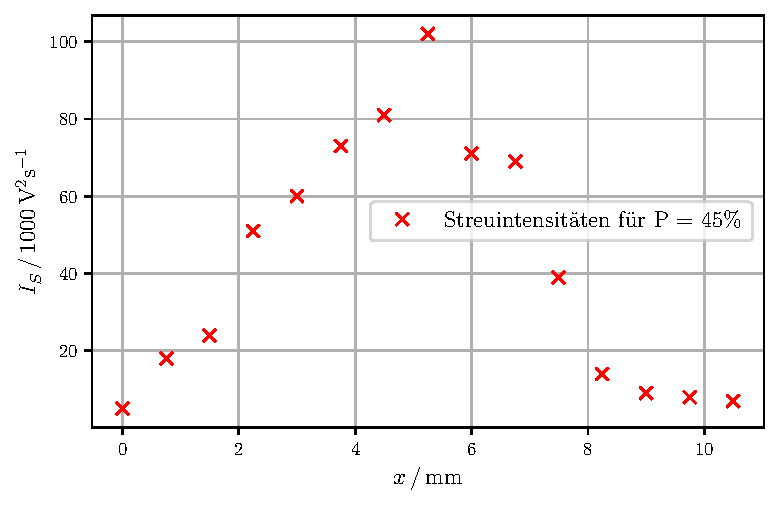
\includegraphics[width=\textwidth]{plot7.pdf}
  \caption{Die Streuintensität für 45$\%$.}
  \label{fig:p7}
  \end{subfigure}

  \caption{Die Strömungsprofile für die jeweiligen Leistungen.}
  \label{fig:profile}
\end{figure}


